% Maerz 2015
% Autor: Mandy Vogel
% Tests 
\documentclass[xcolor={table}]{beamer}
\usetheme{Singapore}

%% \usepackage{listings}
\usepackage{linkimage}

\begin{document}

\title{Non parametric tests for locations}   
\author{Mandy Vogel} 
\date{\today}
%\logo{\includegraphics[scale=0.14]{PIC1}}

\begin{frame}
\titlepage
\end{frame}

\begin{frame}
\frametitle{Table of Contents}\tableofcontents
\end{frame}


\section{Last Session}

\begin{frame}\frametitle{What we've learned}
  \begin{itemize}
  \item different parameters of location and the respective R commands, e.g.
    \begin{itemize}
    \item mean (\texttt{mean()})
    \item trimmed means (\texttt{mean()})
    \item median (\texttt{median()})
    \item quantiles (\texttt{quantile()})
    \item min/max (\texttt{min()/max()})
    \end{itemize}
  \end{itemize}
\end{frame}

\begin{frame}\frametitle{What we've learned}
  \begin{itemize}
  \item different parameters of scale and the respective R commands
    \begin{itemize}
    \item variance and standard deviation (\texttt{var()/sd()})
    \item range (\texttt{range()})
    \item inter quartile range (\texttt{IQR()})
    \end{itemize}
  \end{itemize}
\end{frame}

\begin{frame}\frametitle{What we've learned}
  \begin{itemize}
  \item to specify the way a function works through arguments
    \begin{itemize}
    \item e.g. tell R to ignore missing values (\texttt{mean(x, na.rm=T)})
    \end{itemize}
  \item different kinds of t tests
    \begin{itemize}
    \item one and two sample t test
    \item two sample t tests with and without equal variances (\texttt{t.test(x,y, var.equal=T)})
    \end{itemize}
  \end{itemize}
\end{frame}

\begin{frame}[fragile]\frametitle{What we've learned}
  \begin{itemize}
  \item in R we have two different ways to do a two sample test:
    \begin{itemize}
    \item feed the two vectors of number to the \texttt{t.test()} function: \texttt{t.test(x,y)}
    \item use the formula syntax $values \sim group$, e.g.: 
\begin{verbatim}
  t.test( height ~ sex, data = anthrodata  )
\end{verbatim}
where height is the numeric vector of measurement values, sex is the vector containing the group membership and -- in this case -- both are columns inside a data frame called anthrdata
    \end{itemize}
  \end{itemize}
\end{frame}


\begin{frame}[fragile]\frametitle{Exercise}
  The variable \texttt{sat.m} in the data set \texttt{stud.recs} contains math and verbal SAT scores for a group of students sampled from a larger population. 
  \begin{enumerate}
  \item Load the data from the file \texttt{studrecords.rdata} using the command \texttt{load()}
  \item Test the null hypothesis that the population mean math score (sat.m) is 500 against a two-sided alternative. Would you accept or reject at a 0.05 significance level?
  \item Test the null hypothesis that the mean math score is equal to the mean verbal (sat.v) score against a two sided hypothesis.
  \item Test the null hypothesis that the verbal and the math score is equal in each student.
  \item Extra: The data set contains how many rows? If the data set was very, very largeand representative , what would you expect as result for the latter two tests (as if the SAT test was perfect)?
  \end{enumerate}
\end{frame}

\section{Non parametric tests}

\begin{frame}\frametitle{Intro}
  \begin{itemize}
  \item t-tests relies on a large sample (large means here $n > 30$ for each group) or on the assumption that the parent distribution is normally (or nearly normally) distributed
  \item instead we can do a test on the median
  \item such tests do not make assumptions about the population parameters and are therefore to as \texttt{non-parametric}
  \end{itemize}
\end{frame} 

\subsection{Wilcoxon signed-rank test}
\begin{frame}\frametitle{Wilcoxon test}
    \begin{itemize}
    \item the Wilcoxon tests the location of the median
    \item it is a non-parametric alternative to Student's t test
    \item it is based on the ranks -- and really simple, e.g. for the two sample test: sort your data, give them ranks, sum up the ranks by group, take the smaller sum and look in a table for the appropriate row/column (with ties are dealt with by averaging the appropriate ranks) 
    \item in R it is (not very surprisingly) \texttt{wilcox.test()}
    \item there is also a one and a two sample and a paired version
    \end{itemize}
\end{frame}

\begin{frame}[fragile]\frametitle{Wilcoxon Rank-Sum Test}\footnotesize
\begin{verbatim}
> pre.test <- c(17,12,20,12,20,21,23,10,15,17,18,18)
> post.test <- c(19,25,18,18,26,19,27,14,20,22,16,18)
> wilcox.test(pre.test,post.test,paired = T)

	Wilcoxon signed rank test with continuity correction

data:  pre.test and post.test
V = 7.5, p-value = 0.02527
alternative hypothesis: true location shift is not equal to 0

Warning messages:
1: In wilcox.test.default(pre.test, post.test, paired = T) :
  kann bei Bindungen keinen exakten p-Wert Berechnen
2: In wilcox.test.default(pre.test, post.test, paired = T) :
  kann den exakten p-Wert bei Nullen nicht berechnen
\end{verbatim}
\end{frame}

\begin{frame}[fragile]\frametitle{Wilcoxon Rank-Sum Test}
\begin{itemize}
\item the non-parametric test is much more appropriate when the errors are not normal, 
\item can be more powerful if the distribution is strongly skewed by the presence of outliers
\item typically, as here, the t-test will give the lower p-value, so the Wilcoxon test is said to be conservative: if a difference is significant under a Wilcoxon test it would have been even more significant under a t-test.
\end{itemize}
\end{frame}

\begin{frame}\frametitle{Exercise}
  \begin{enumerate}
  \item load the data frame normtemp from the file temperature.rdata; it contains the body temperature of several individuals, the gender and the heart rate
  \item test if the temperature is different in male (coded as 1) and female (coded as 2), use the appropriate test.
  \item test again, compare the results of the t test and the wilcoxon.
  \item plot the respective boxplots!
  \end{enumerate}
\end{frame}

\section{ggplot2}
\subsection{Another layer}
\begin{frame}[fragile]\frametitle{Another layer}
  \begin{itemize}
  \item after we've produced our basic plot we can add another layer
  \item so e.g. we can try to add points by adding a point layer -- \texttt{geom\_point()}
  \end{itemize}\small
\begin{verbatim}
> ggplot(normtemp, aes(x = factor(gender), y = temperature)) +
+     geom_boxplot() +
+     geom_point()  
\end{verbatim}
which results in:
\end{frame}

\begin{frame}\frametitle{Another layer}
  \begin{center}
    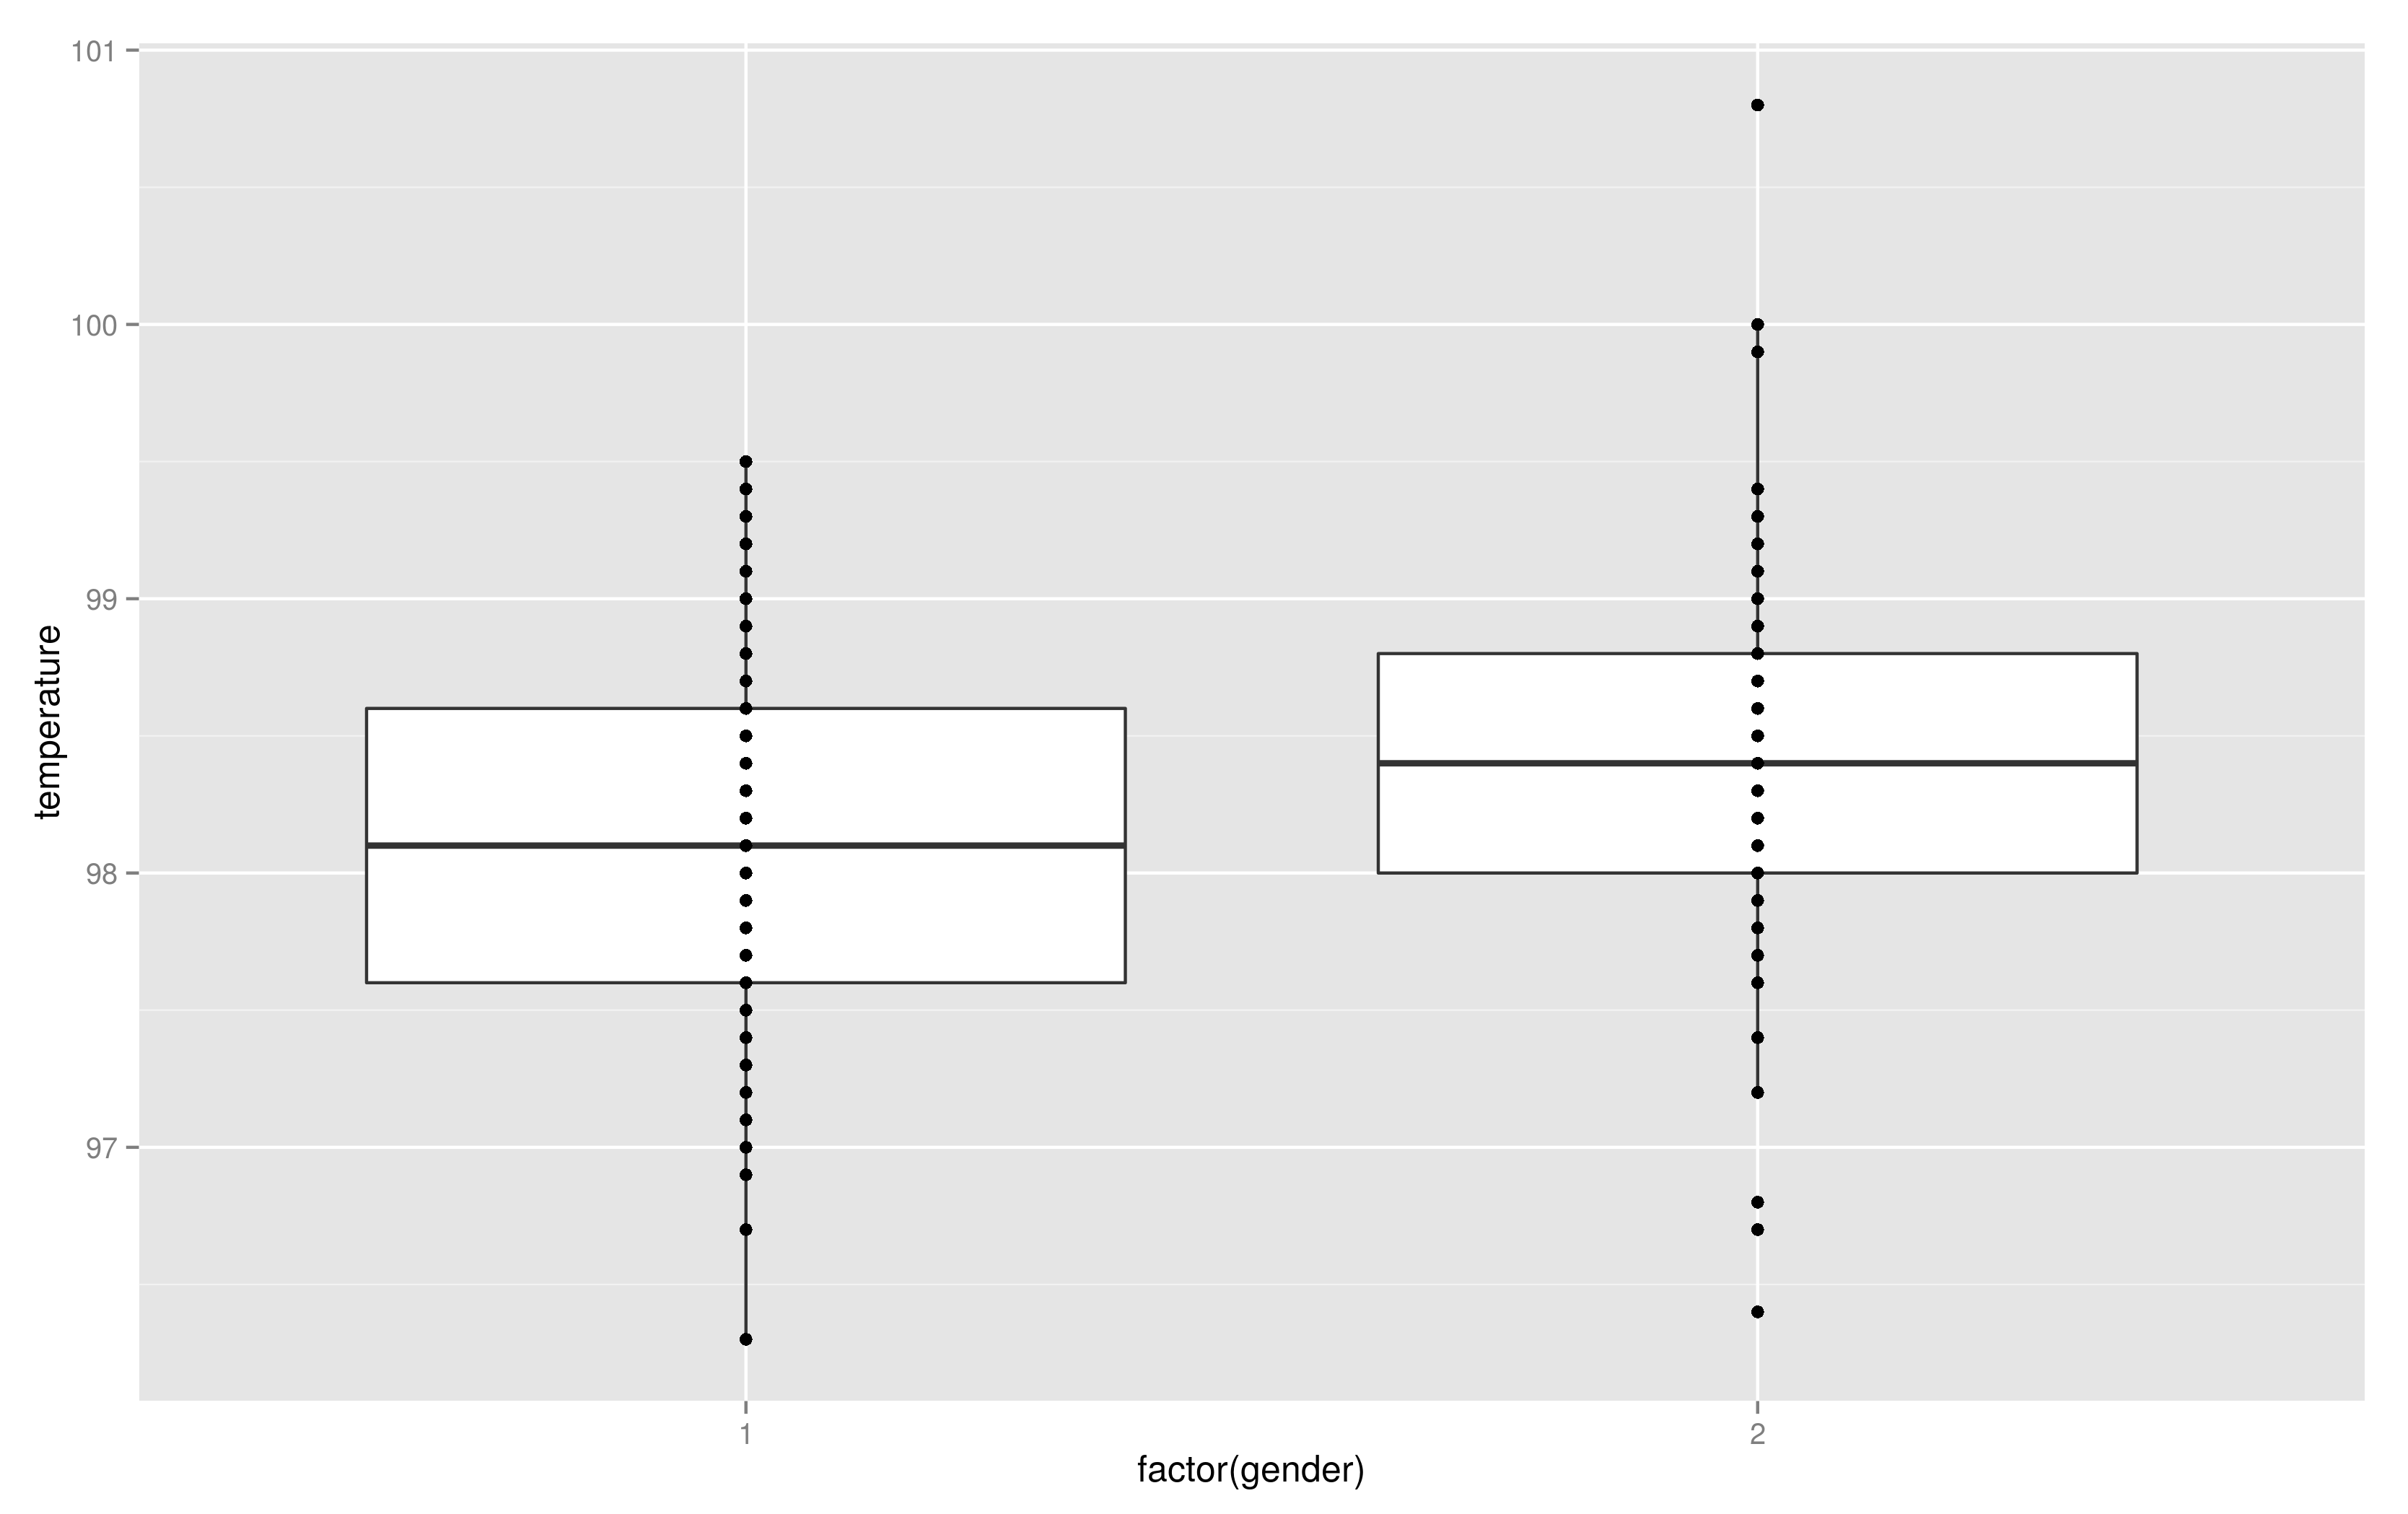
\includegraphics[width=9cm]{boxplotpoint.png}
  \end{center}
\end{frame}

\begin{frame}[fragile]\frametitle{Another layer}
  \begin{itemize}
  \item so what we see here?
  \item every point in the figure represents \textit{at least} one point in the data
  \item one way to overcome this problem and to show \texttt{all} points is to use \texttt{geom\_jitter()} instead of the point geom; this adds a little random noise to the points
  \end{itemize}\small
\begin{verbatim}
> ggplot(normtemp, aes(x = factor(gender), y = temperature)) +
+     geom_boxplot() +
+     geom_jitter()  
\end{verbatim}
which results in:
\end{frame}

\begin{frame}\frametitle{Another layer}
  \begin{center}
    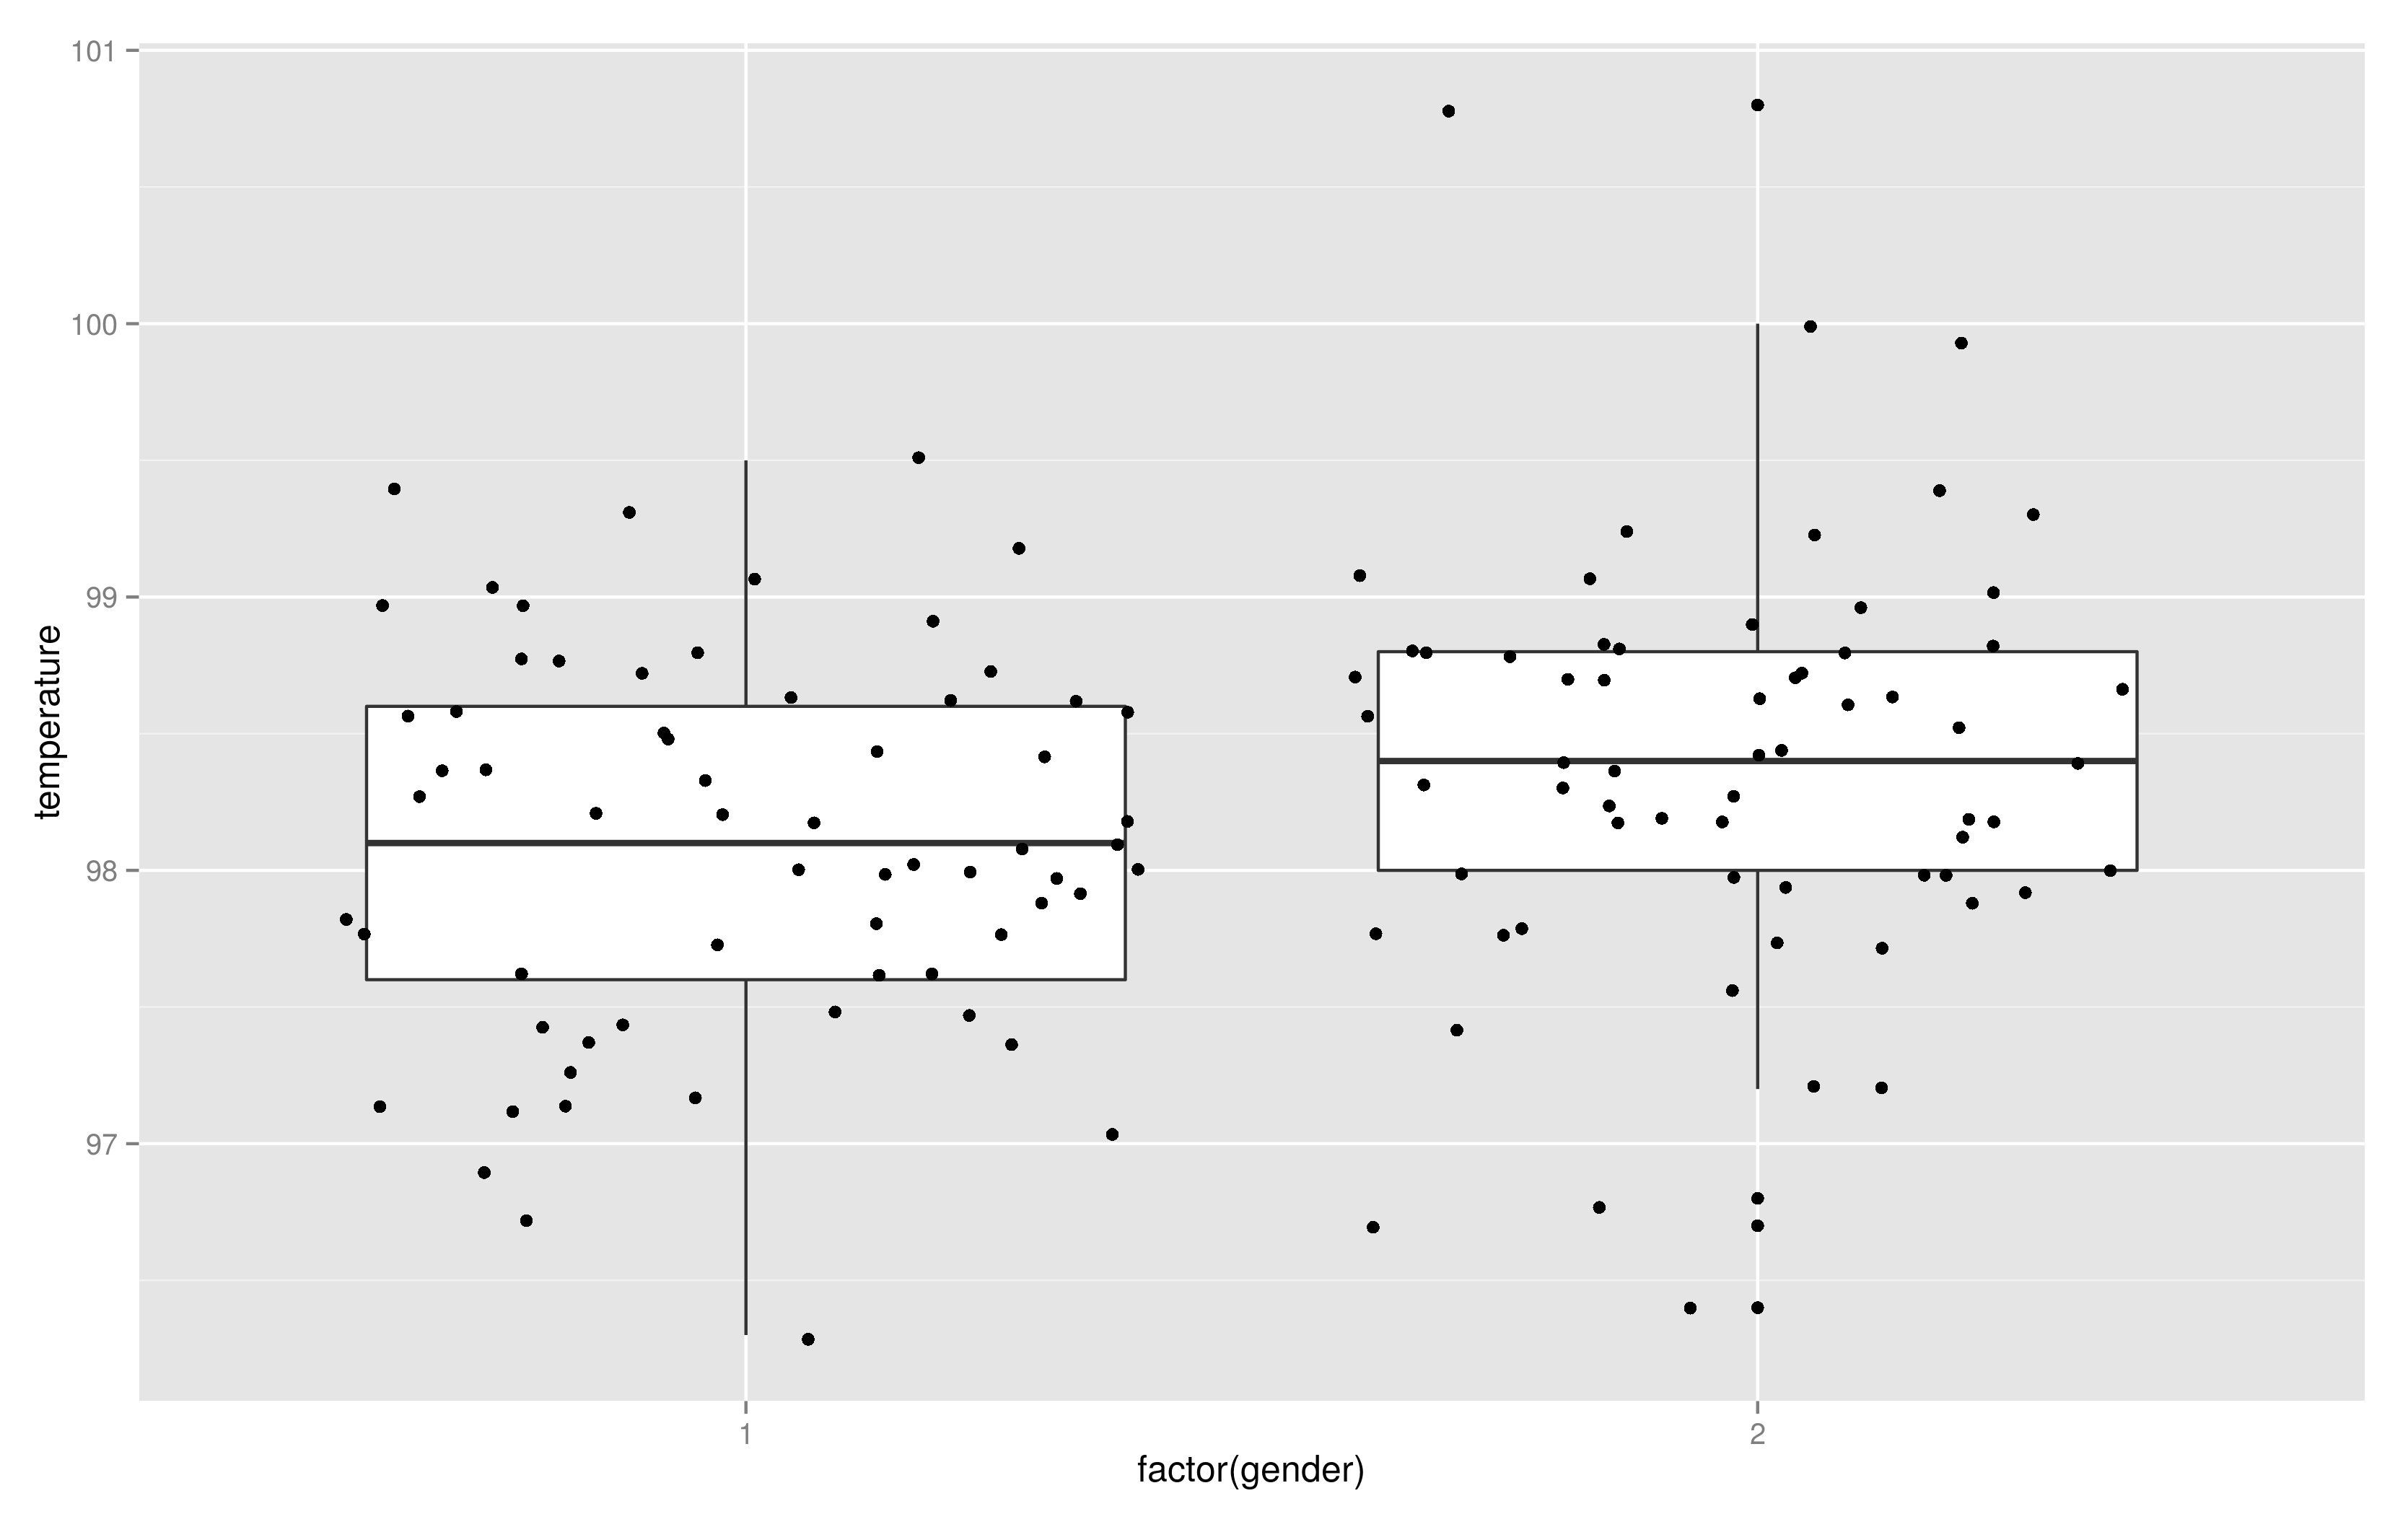
\includegraphics[width=9cm]{boxplotjitter.png}
  \end{center}
\end{frame}

\begin{frame}[fragile]\frametitle{Another layer}
  \begin{itemize}
  \item you can specify the scale of jitter using the \texttt{width} and \texttt{height} arguments inside the position argument
  \end{itemize}\small
\begin{verbatim}
> ggplot(normtemp, aes(x = factor(gender), y = temperature)) +
+     geom_boxplot() +
+     geom_jitter(position=position_jitter(width=0.1))
\end{verbatim}
which results in:
\end{frame}

\begin{frame}\frametitle{Another layer}
  \begin{center}
    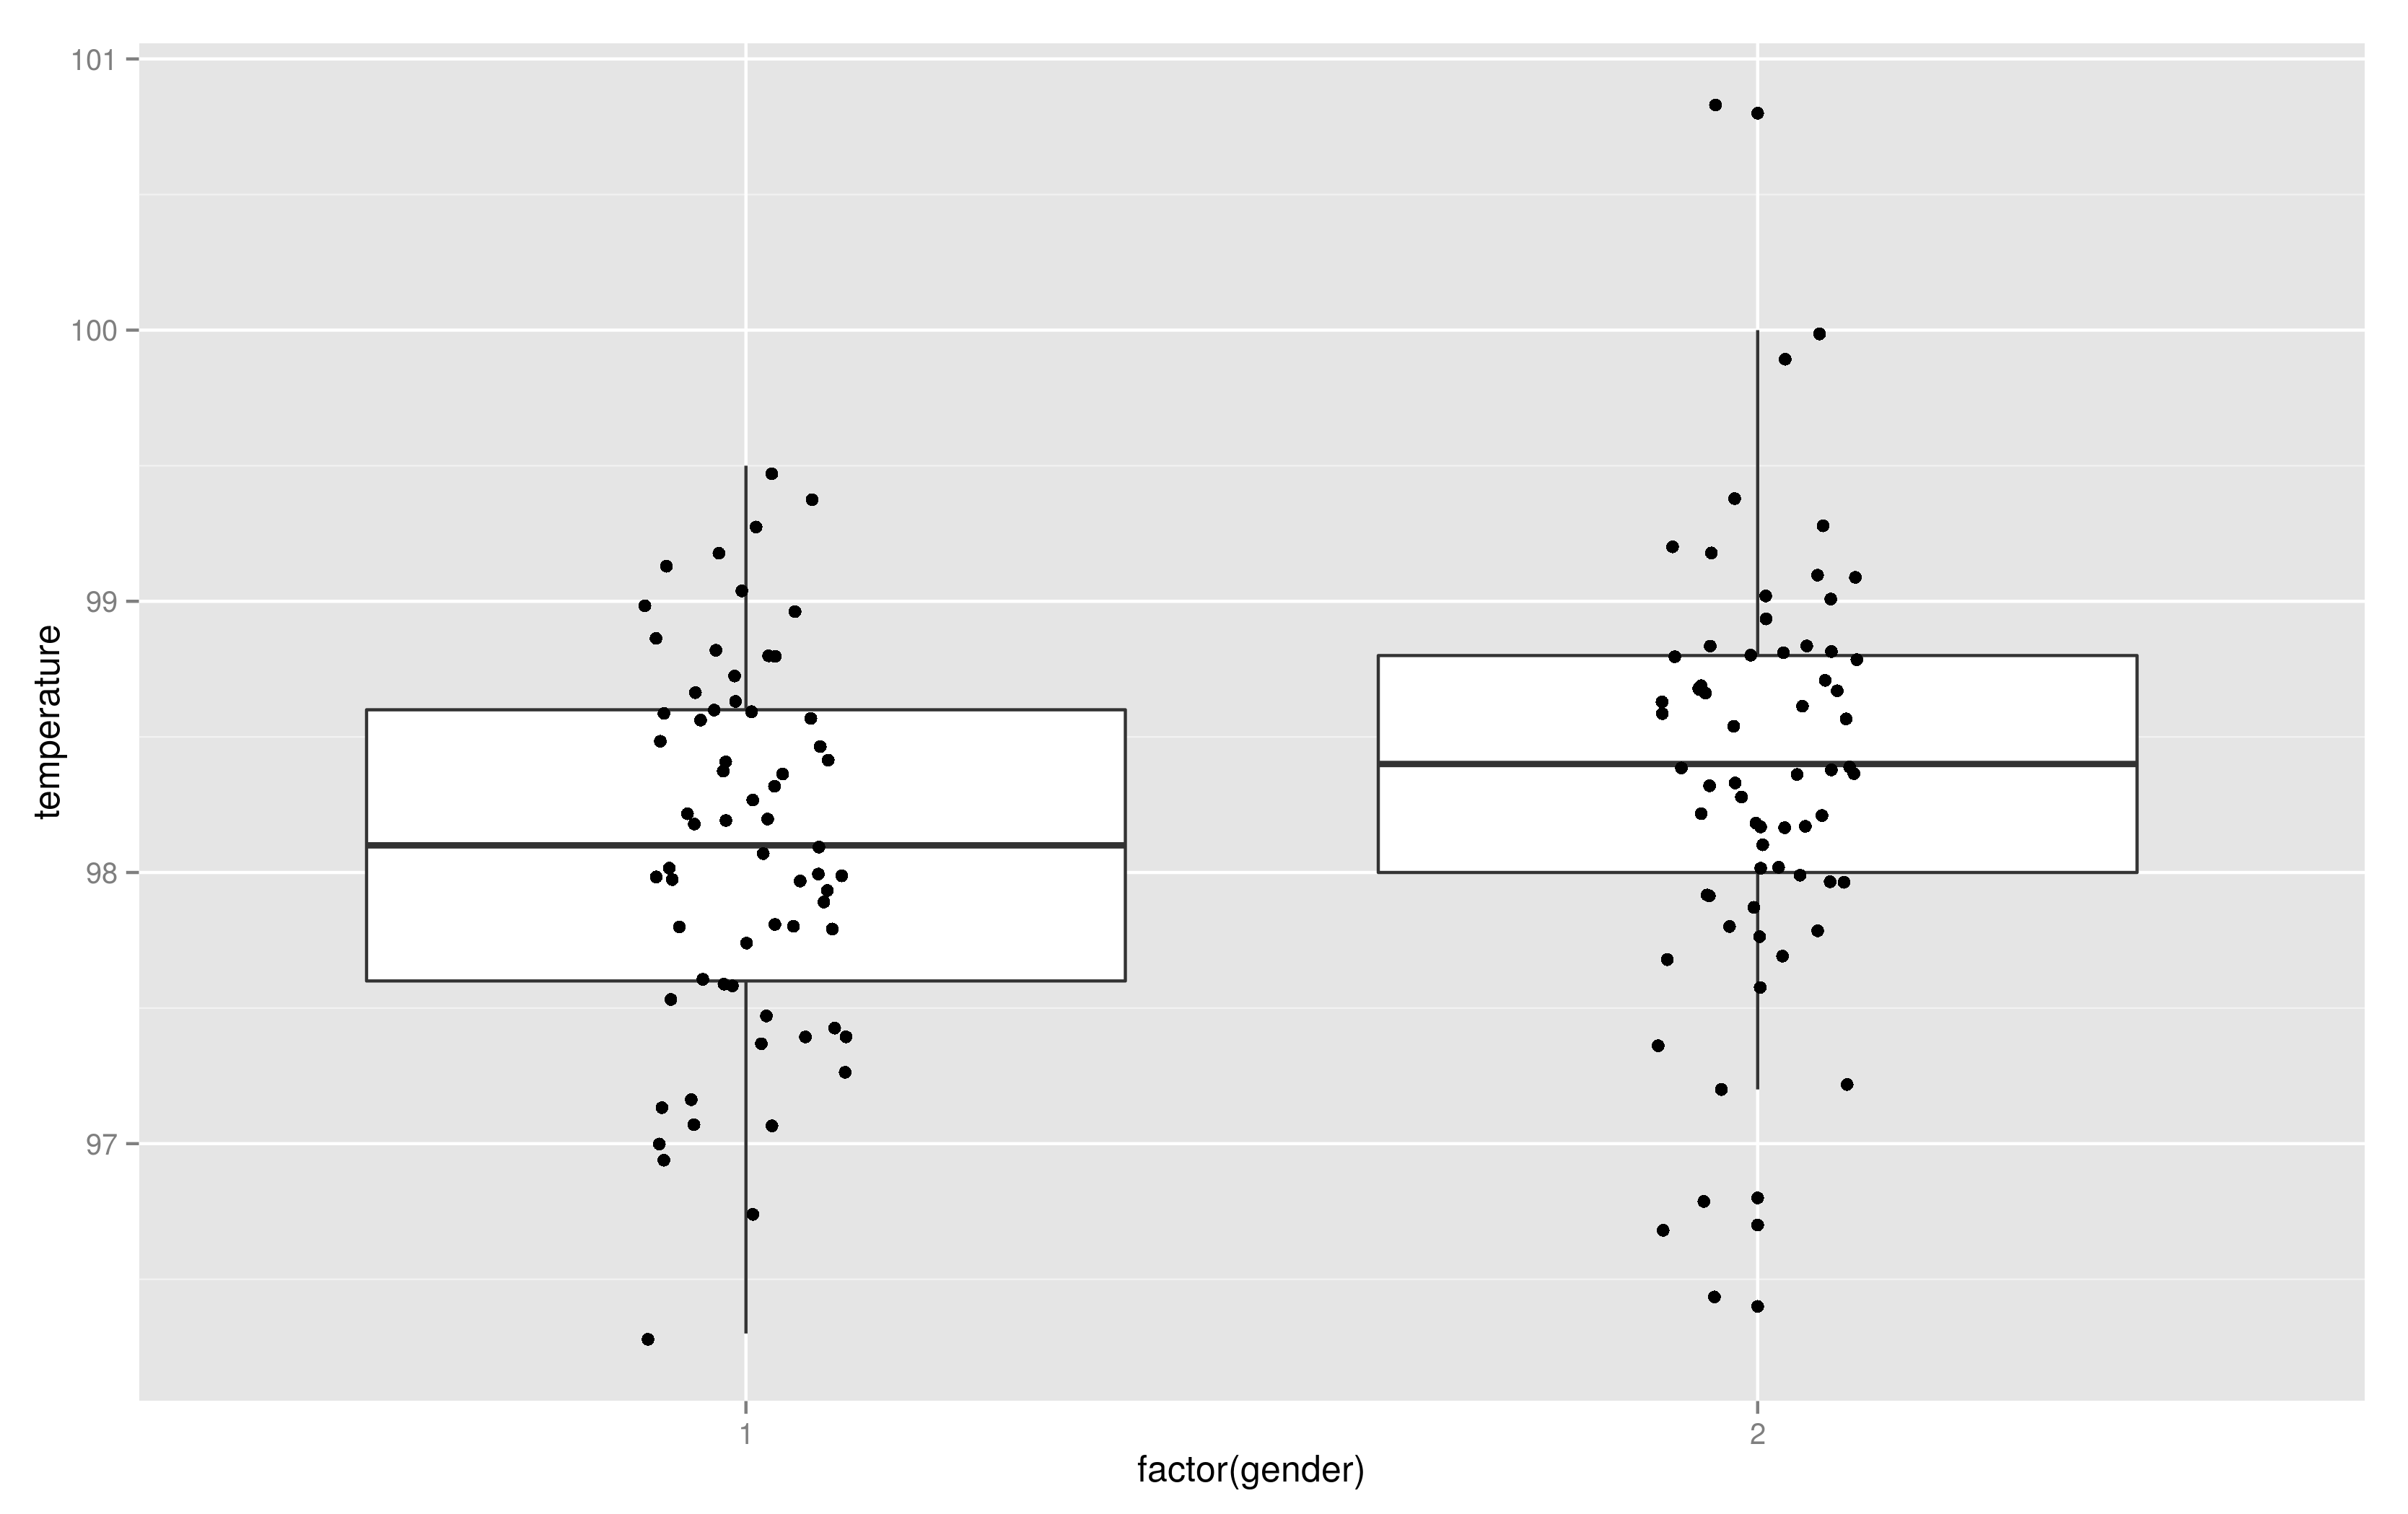
\includegraphics[width=9cm]{boxplotjitter2.png}
  \end{center}
\end{frame}


\begin{frame}[fragile]\frametitle{Another layer}
  \begin{itemize}
  \item up till now we plotted the points as they are but what if we want to plot not all points but just one point representing the mean
  \item so we have to use an \textit{statistic}, a summary statistic or better, we have to make our \texttt{geom\_point()} using it
  \end{itemize}\small
\begin{verbatim}
> ggplot(normtemp, aes(x = factor(gender), y = temperature)) +
+     geom_boxplot() +
+     geom_point(stat = "summary", fun.y = "mean")
\end{verbatim}
which results in:
\end{frame}

\begin{frame}\frametitle{Another layer}
  \begin{center}
    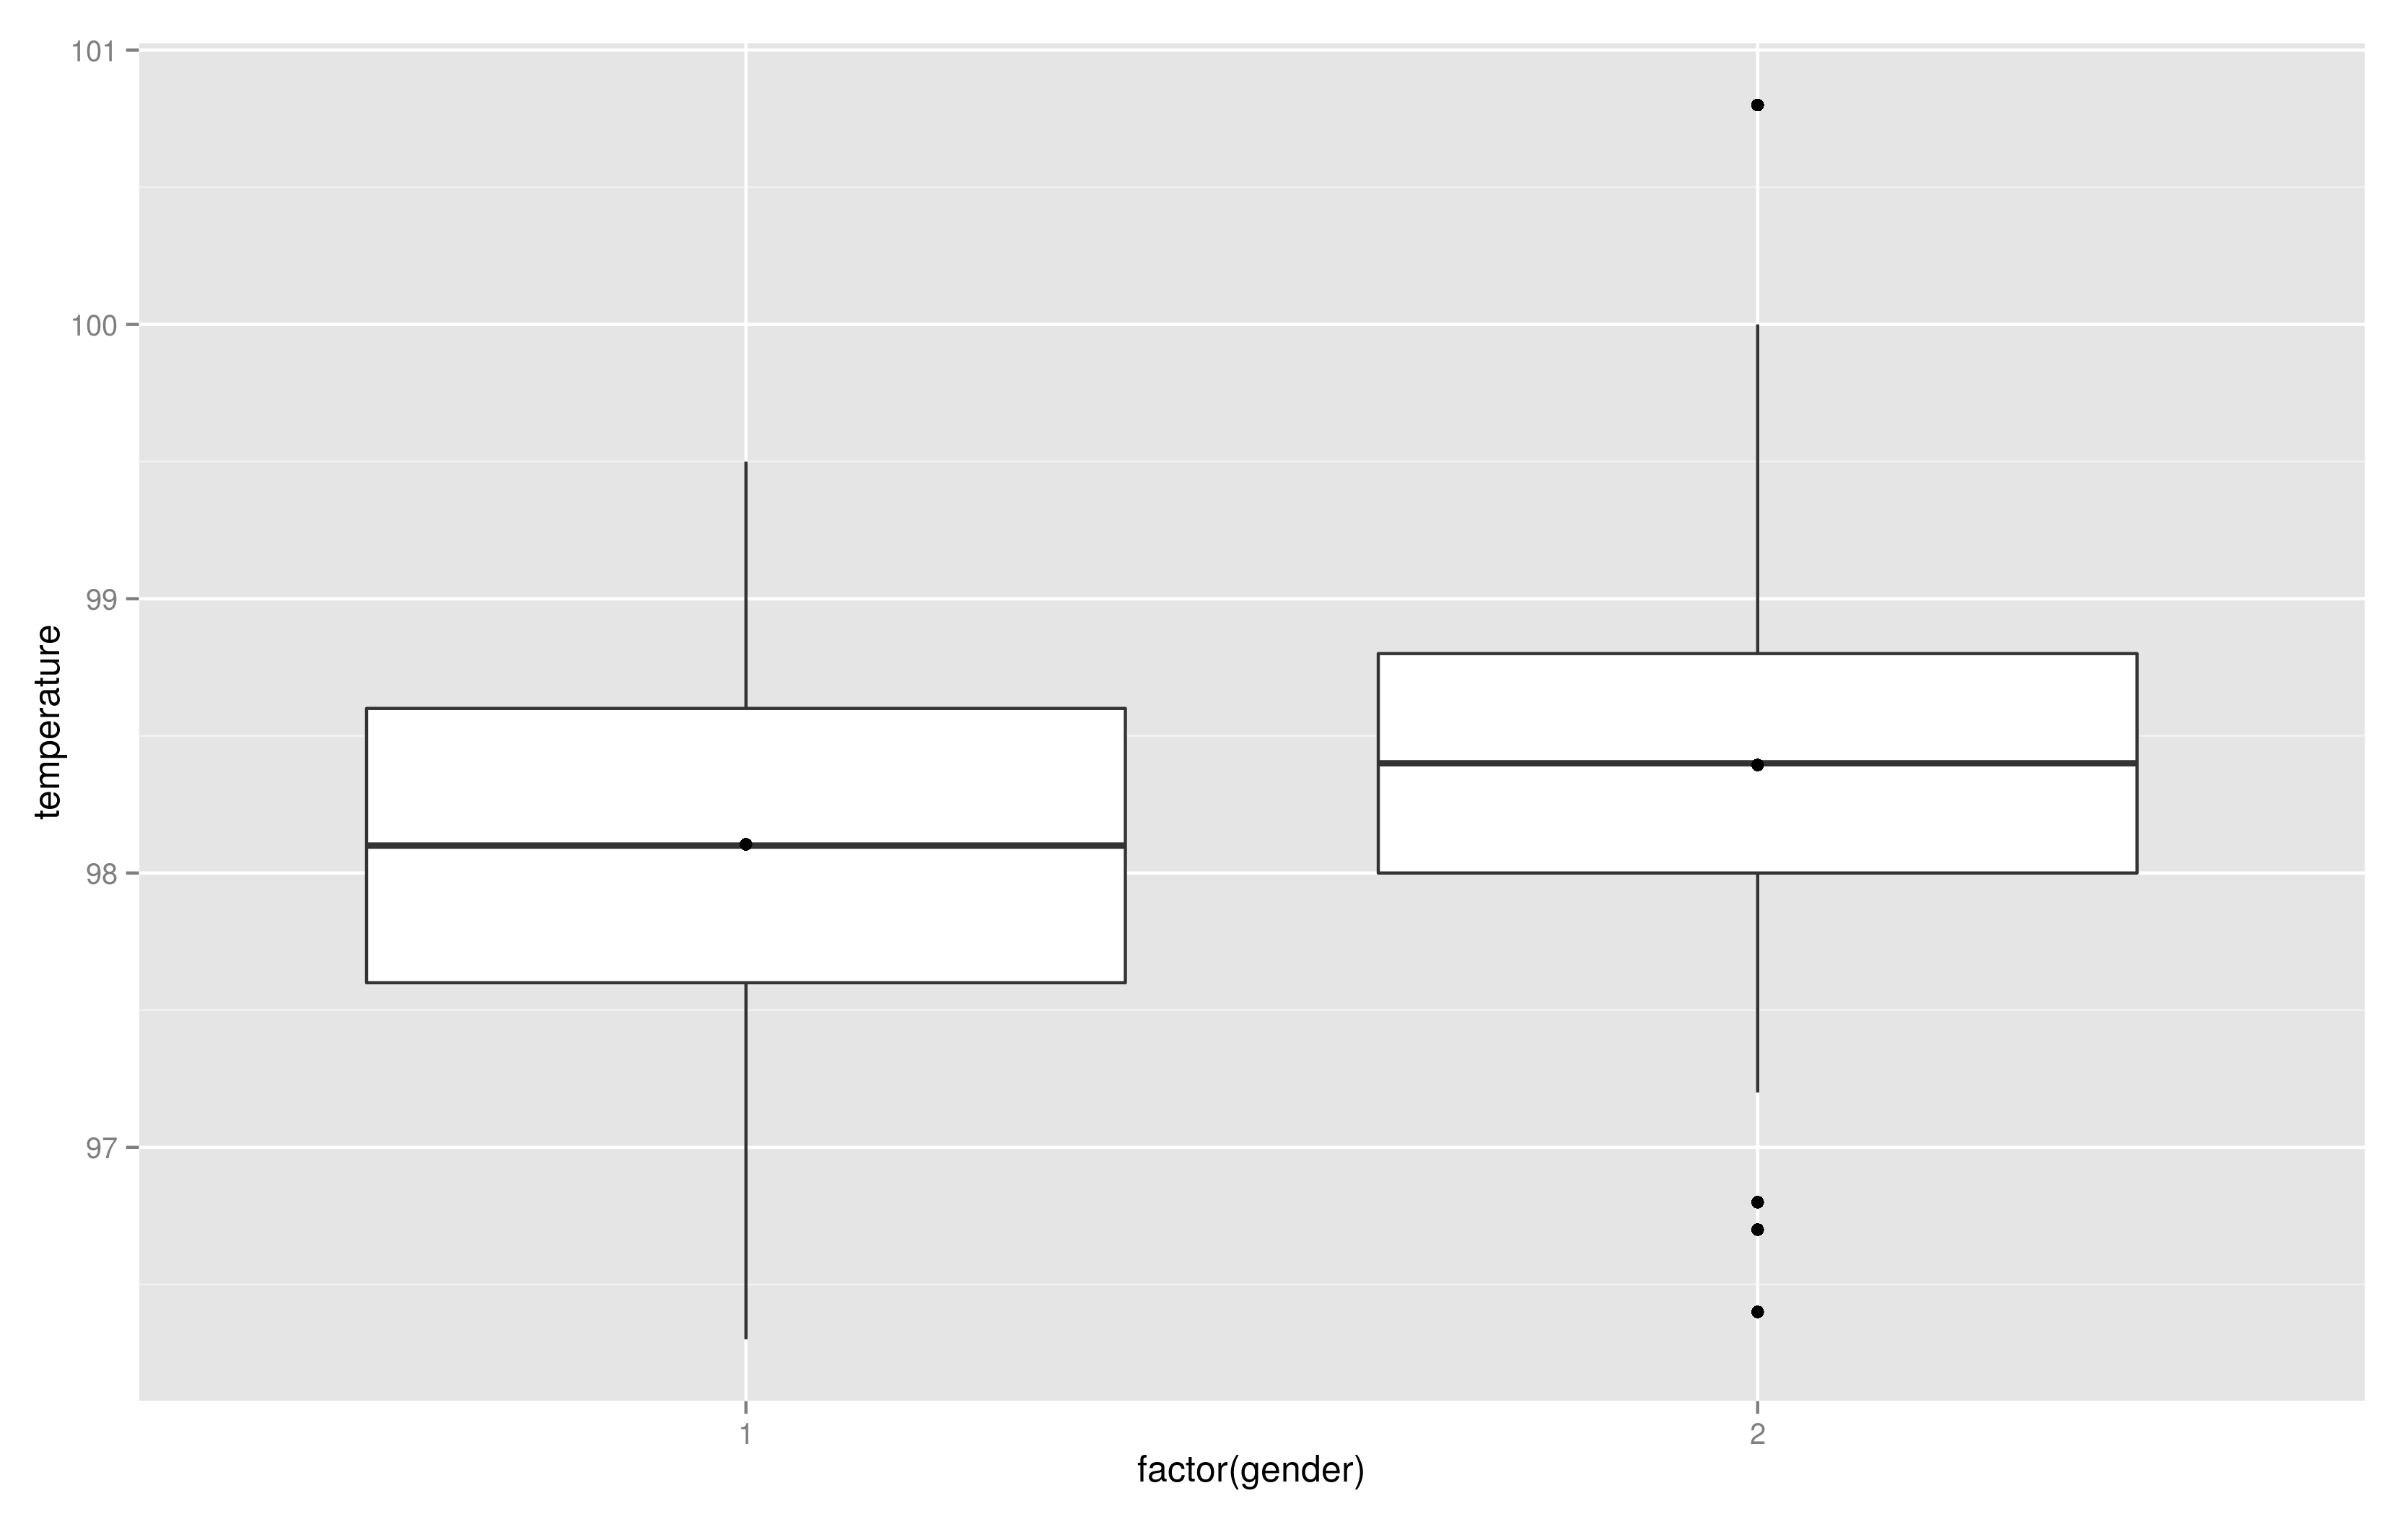
\includegraphics[width=9cm]{boxplotmean.png}
  \end{center}
\end{frame}

\begin{frame}[fragile]\frametitle{Another layer}
  \begin{itemize}
  \item and now a little larger and red
  \end{itemize}\small
\begin{verbatim}
> ggplot(normtemp, aes(x = factor(gender), y = temperature)) +
+     geom_boxplot() +
+     geom_point(stat = "summary", fun.y = "mean",
+                size = 5, colour = "red"))
\end{verbatim}
which results in:
\end{frame}

\begin{frame}\frametitle{Another layer}
  \begin{center}
    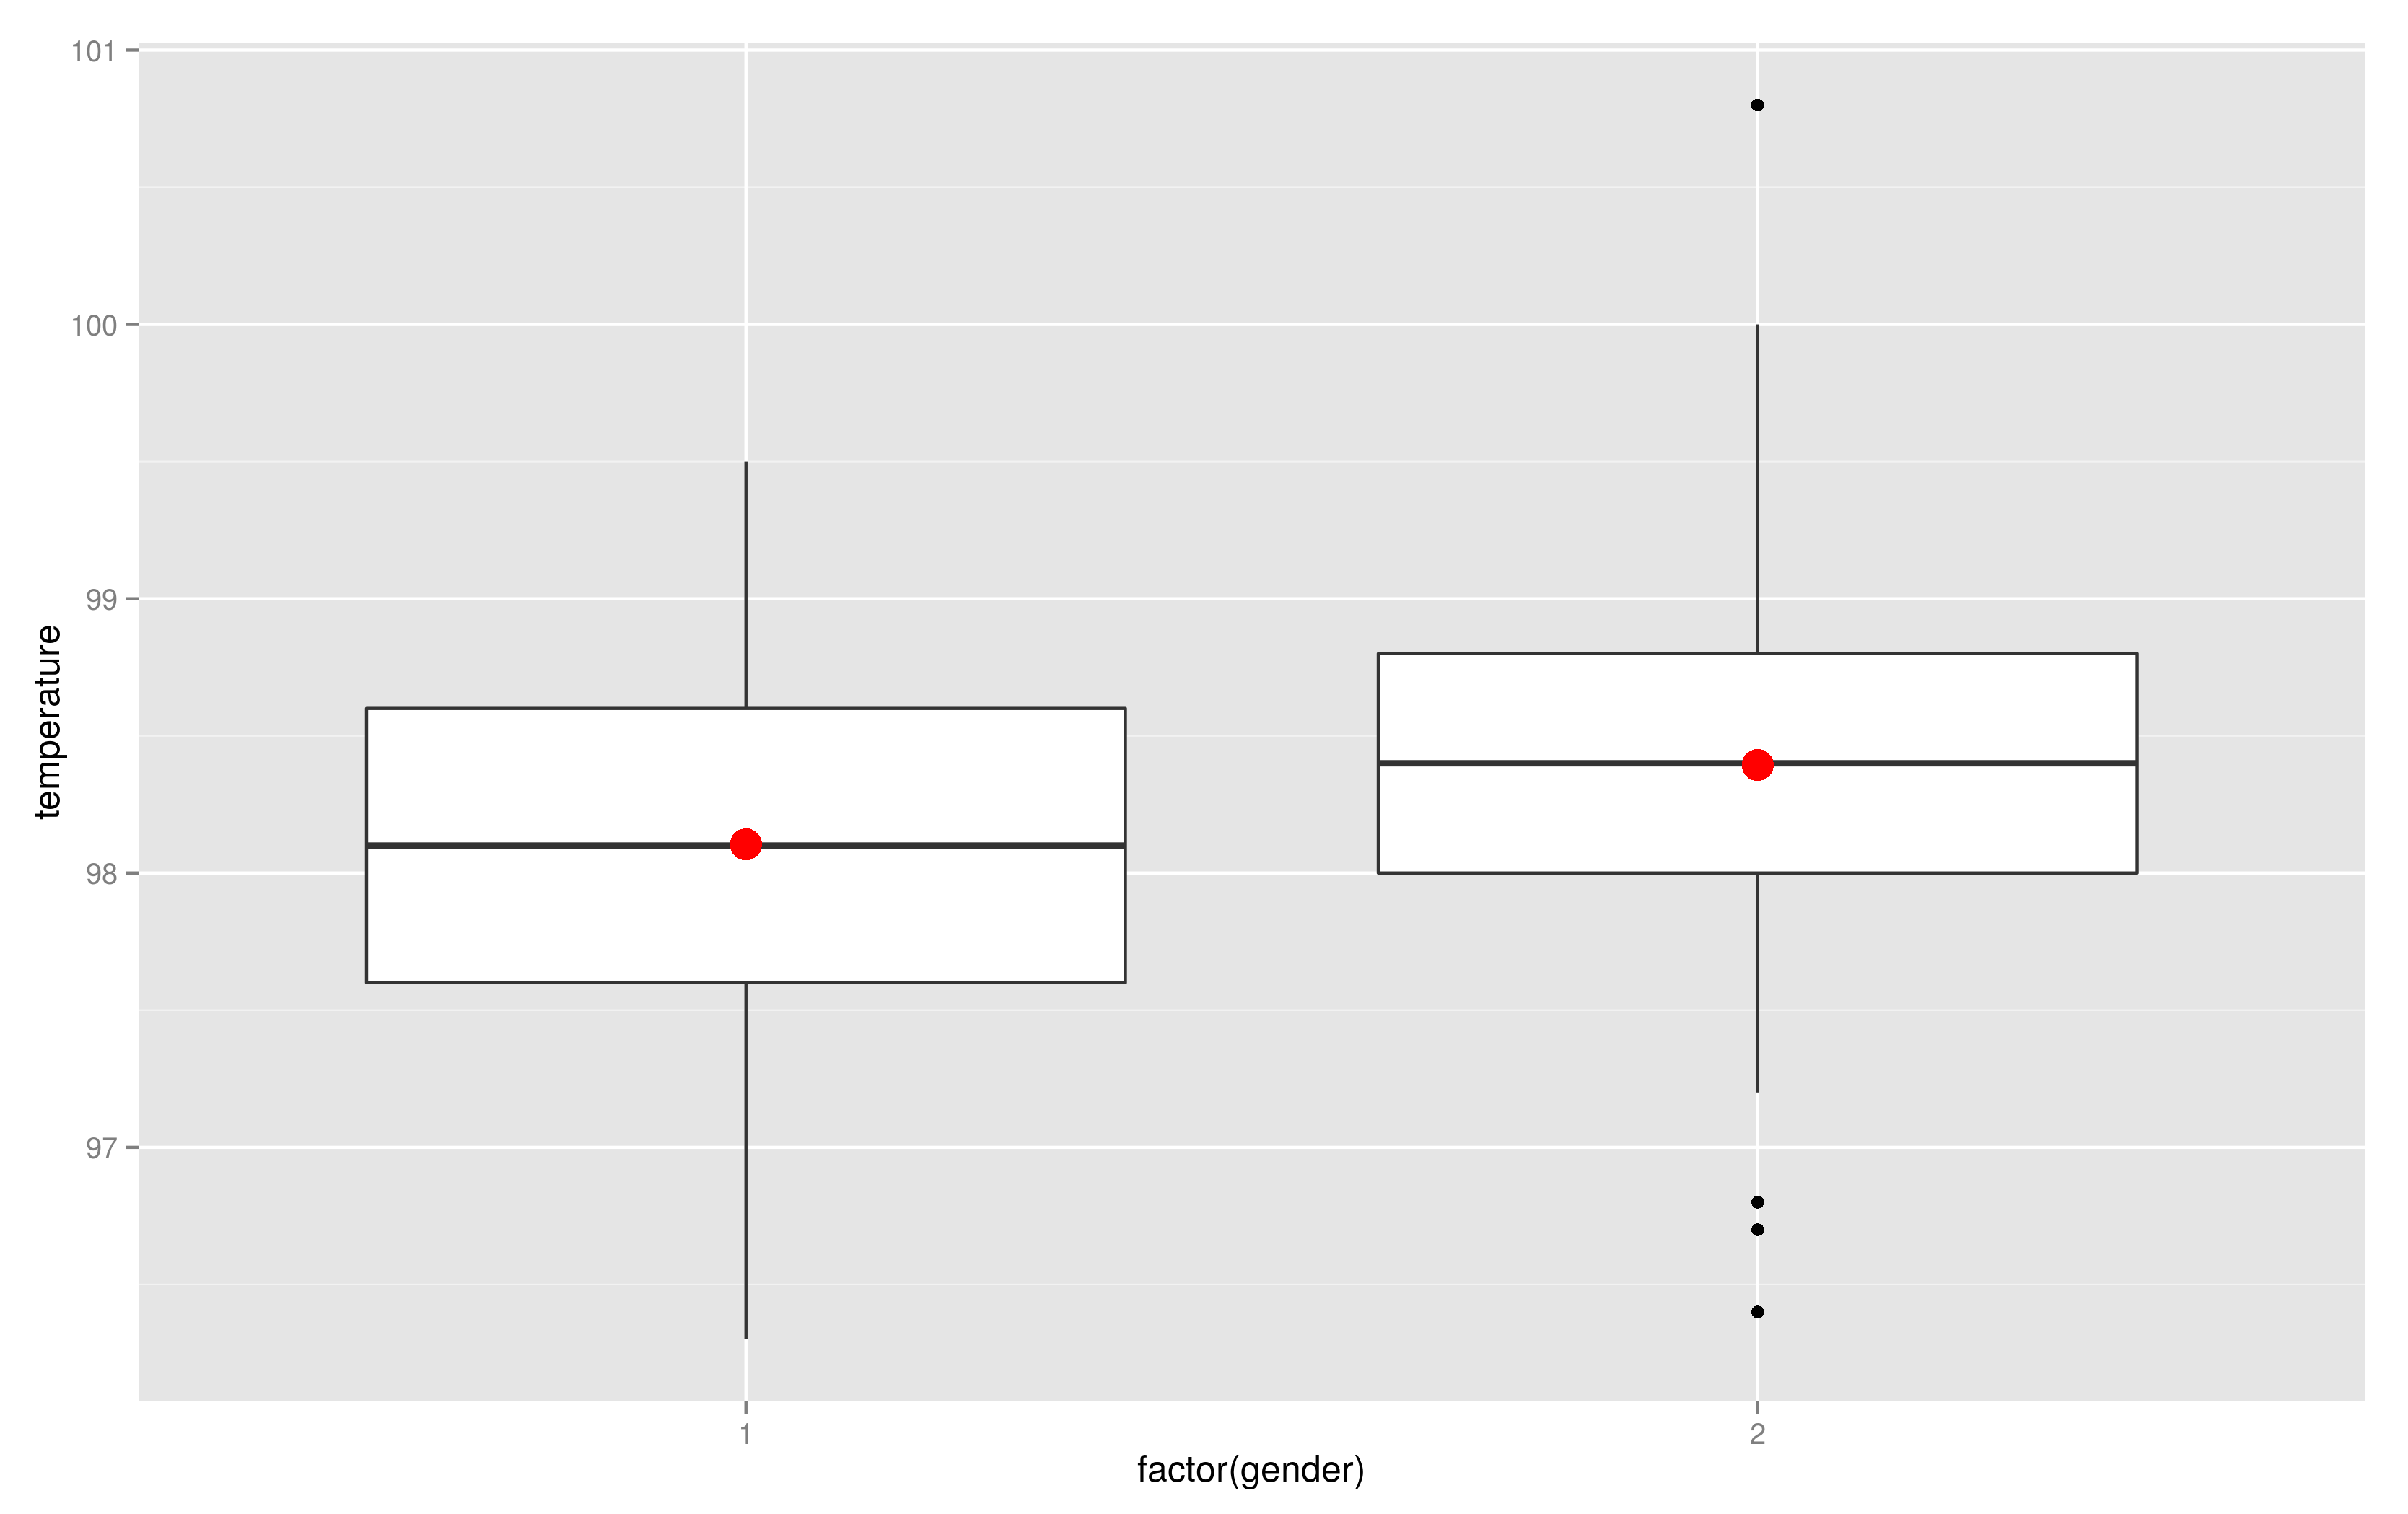
\includegraphics[width=9cm]{boxplotmean2.png}
  \end{center}
\end{frame}


\begin{frame}[allowframebreaks]\frametitle{Exercises}
  \begin{enumerate}
  \item load the data set \texttt{GaltonFamilies} from the package HistData 
    \begin{itemize}
    \item you may have to install HistData (it depends)
    \item use \texttt{library()} or \texttt{require()} to load the package
    \end{itemize}
    \item make a boxplot of \texttt{childHeight} dependent on gender
    \item add the means using \texttt{geom\_point()}
    \item do the respective t-test: what is the (trivial) null hypothesis, what is appropriate test, what is the test result and what is the conclusion?
  \end{enumerate}
\end{frame}


\subsection{Bivariate Data}
\begin{frame}[fragile,allowframebreaks]\frametitle{Scatter plots}
  \begin{itemize}
  \item up to now we only visualized univariate numerical data but we already used a central geom for visualizing bivariate data 
  \item to produce a scatter plot we use \texttt{geom\_point()} with the aesthetics \texttt{aes(x = variable1, y = variable2)}
  \item we can customize the size (\texttt{size}), shape (\texttt{shape}), colour(\texttt{colour} and \texttt{fill}), and transparency (\texttt{alpha}) of the points 
  \begin{center}
    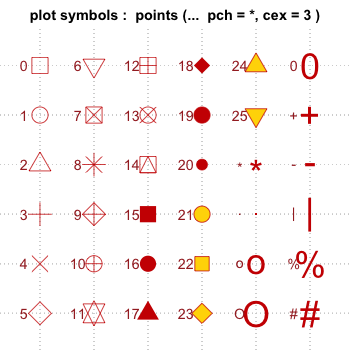
\includegraphics[width=6cm]{shapes.png}
  \end{center}
  \end{itemize}
\end{frame}

\begin{frame}[fragile]\frametitle{Scatter plots}
\small
\begin{verbatim}
> ggplot(GaltonFamilies, aes(x=mother,y=father)) +
+     geom_point()
\end{verbatim}
which results in:
\end{frame}


\begin{frame}\frametitle{Scatter plots}
  \begin{center}
    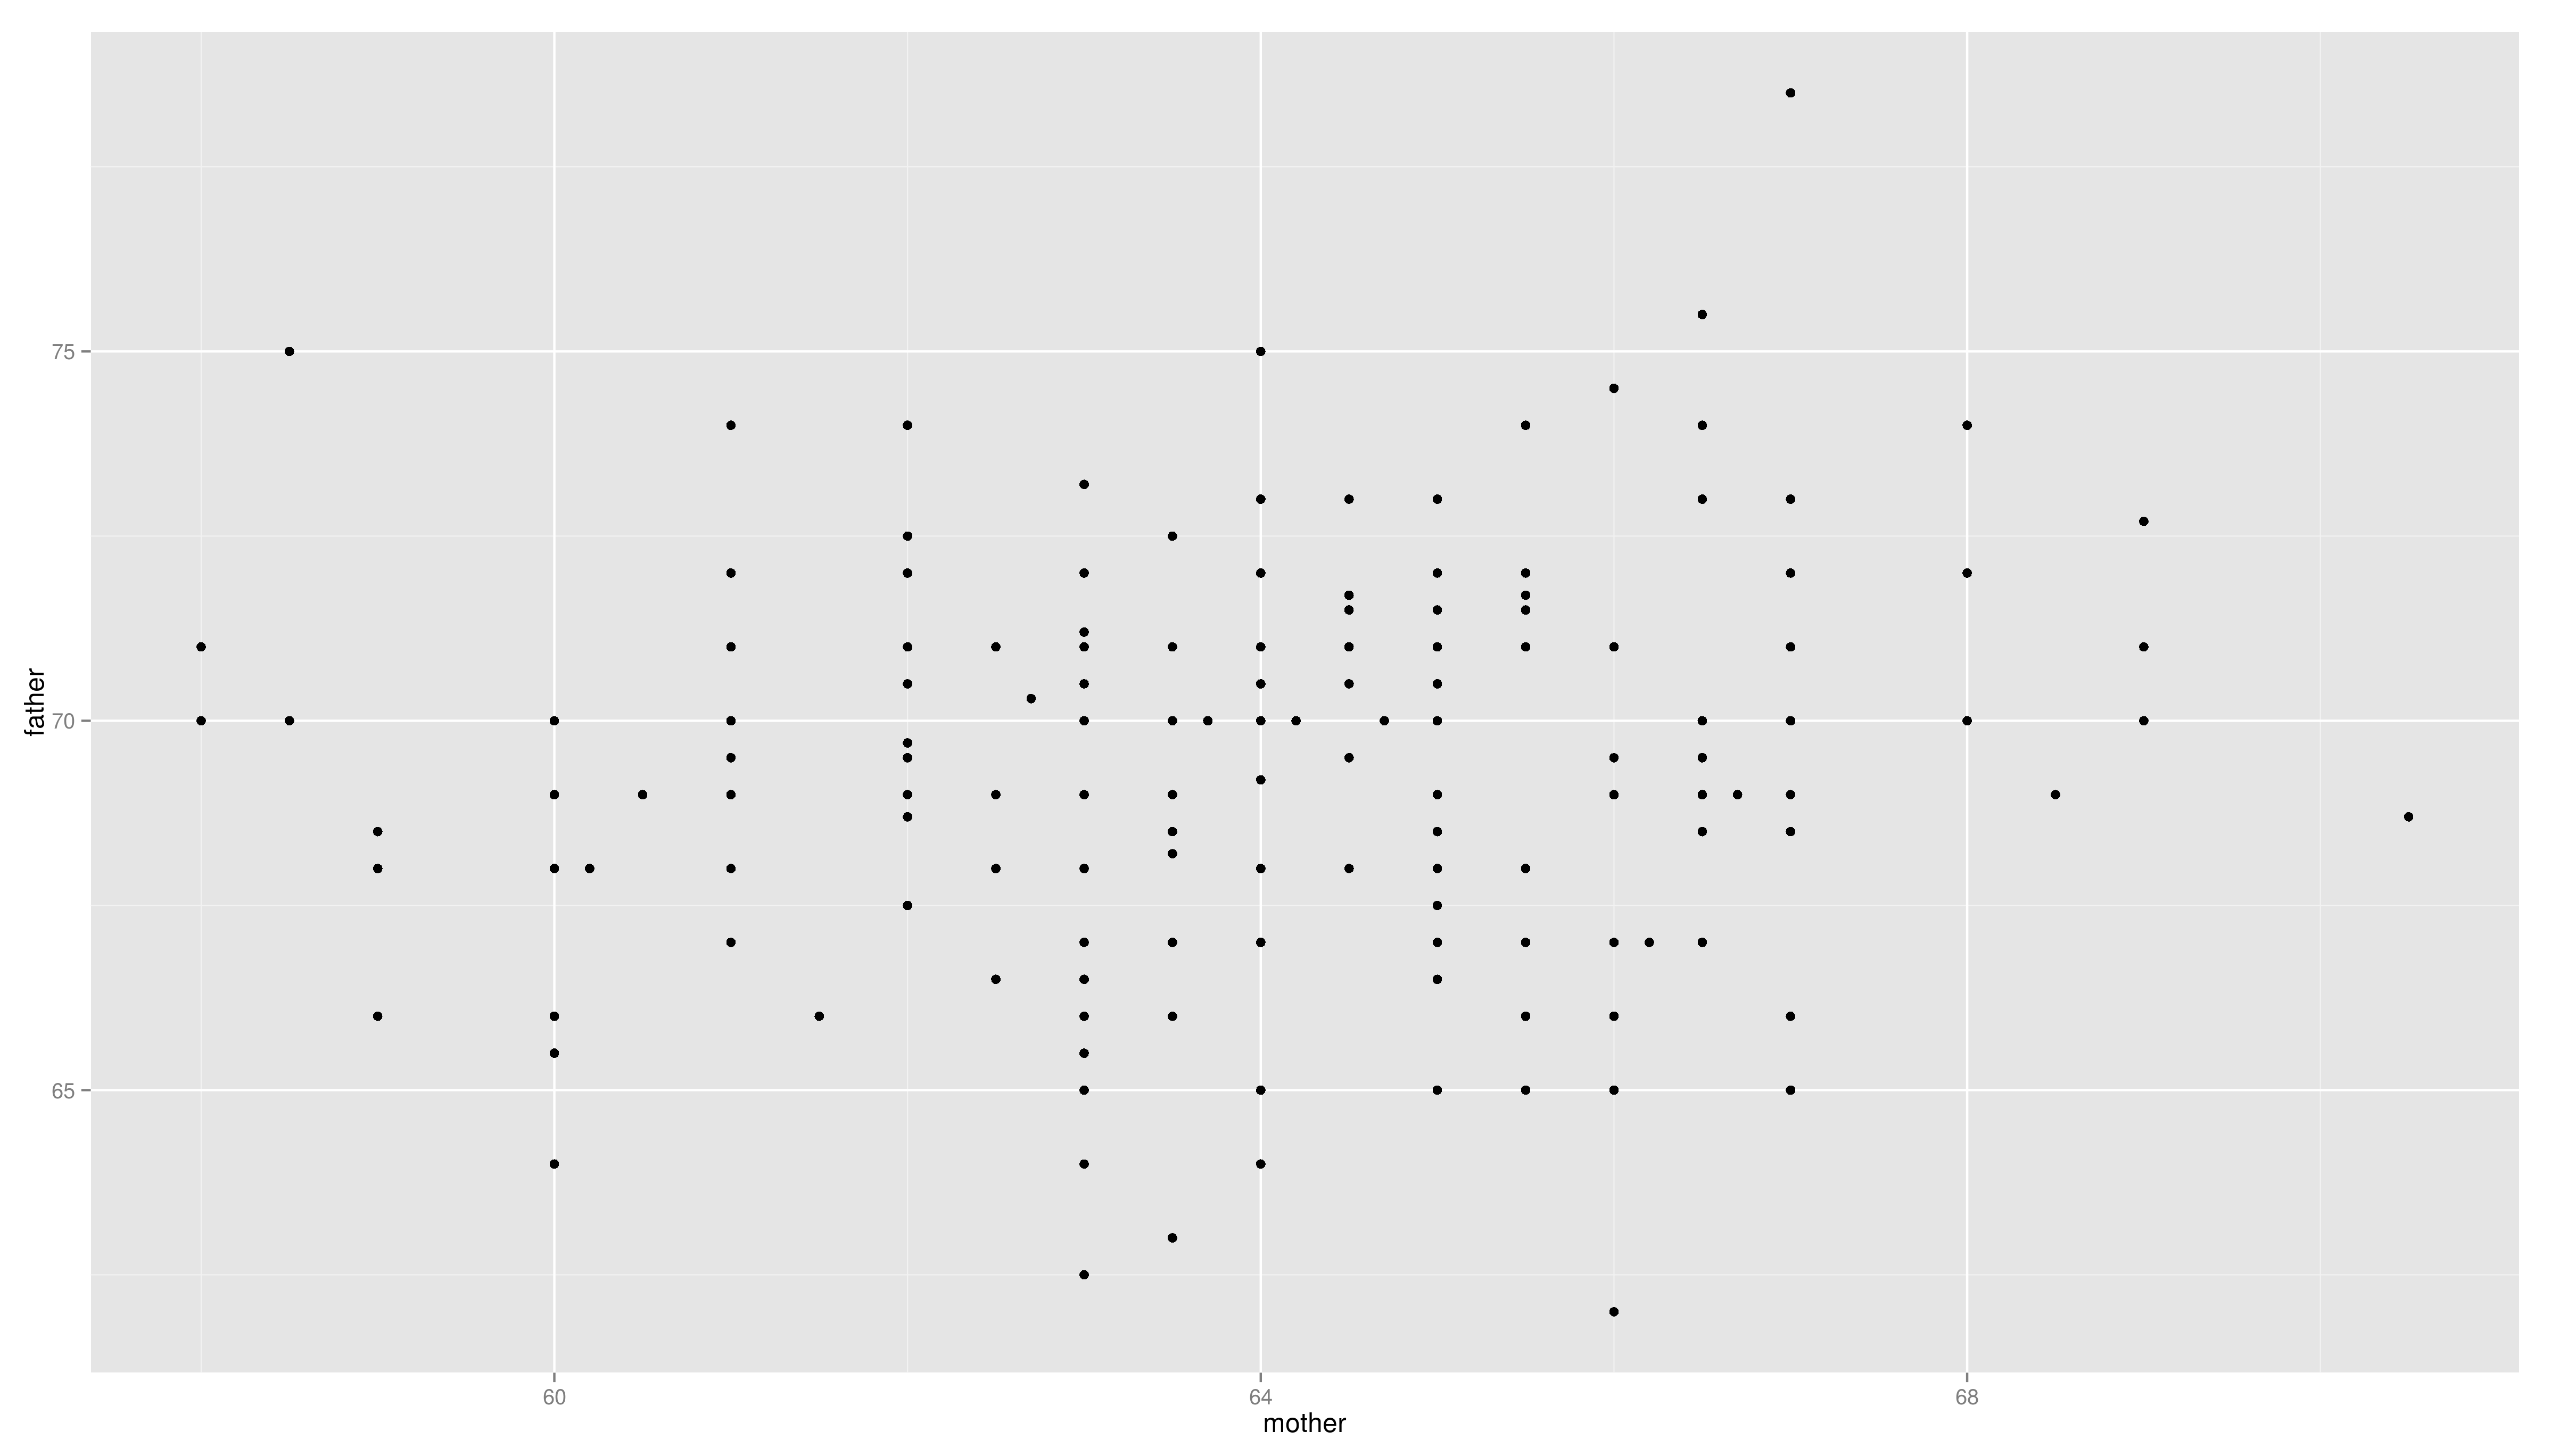
\includegraphics[width=9cm]{scatter.png}
  \end{center}
\end{frame}

\begin{frame}[fragile]\frametitle{Adding trend lines}
  \begin{itemize}
  \item a trend line is a statistical summary of a bivariate relationship
  \item there are many different trend lines that can be added to a scatterplot
  \item they are easily added through \texttt{geom\_smooth()}
  \end{itemize}\small
\begin{verbatim}
> ggplot(GaltonFamilies, aes(x=mother,y=father)) +
+     geom_point()
\end{verbatim}
which results in:
\end{frame}


\begin{frame}\frametitle{Adding trend lines}
  \begin{center}
    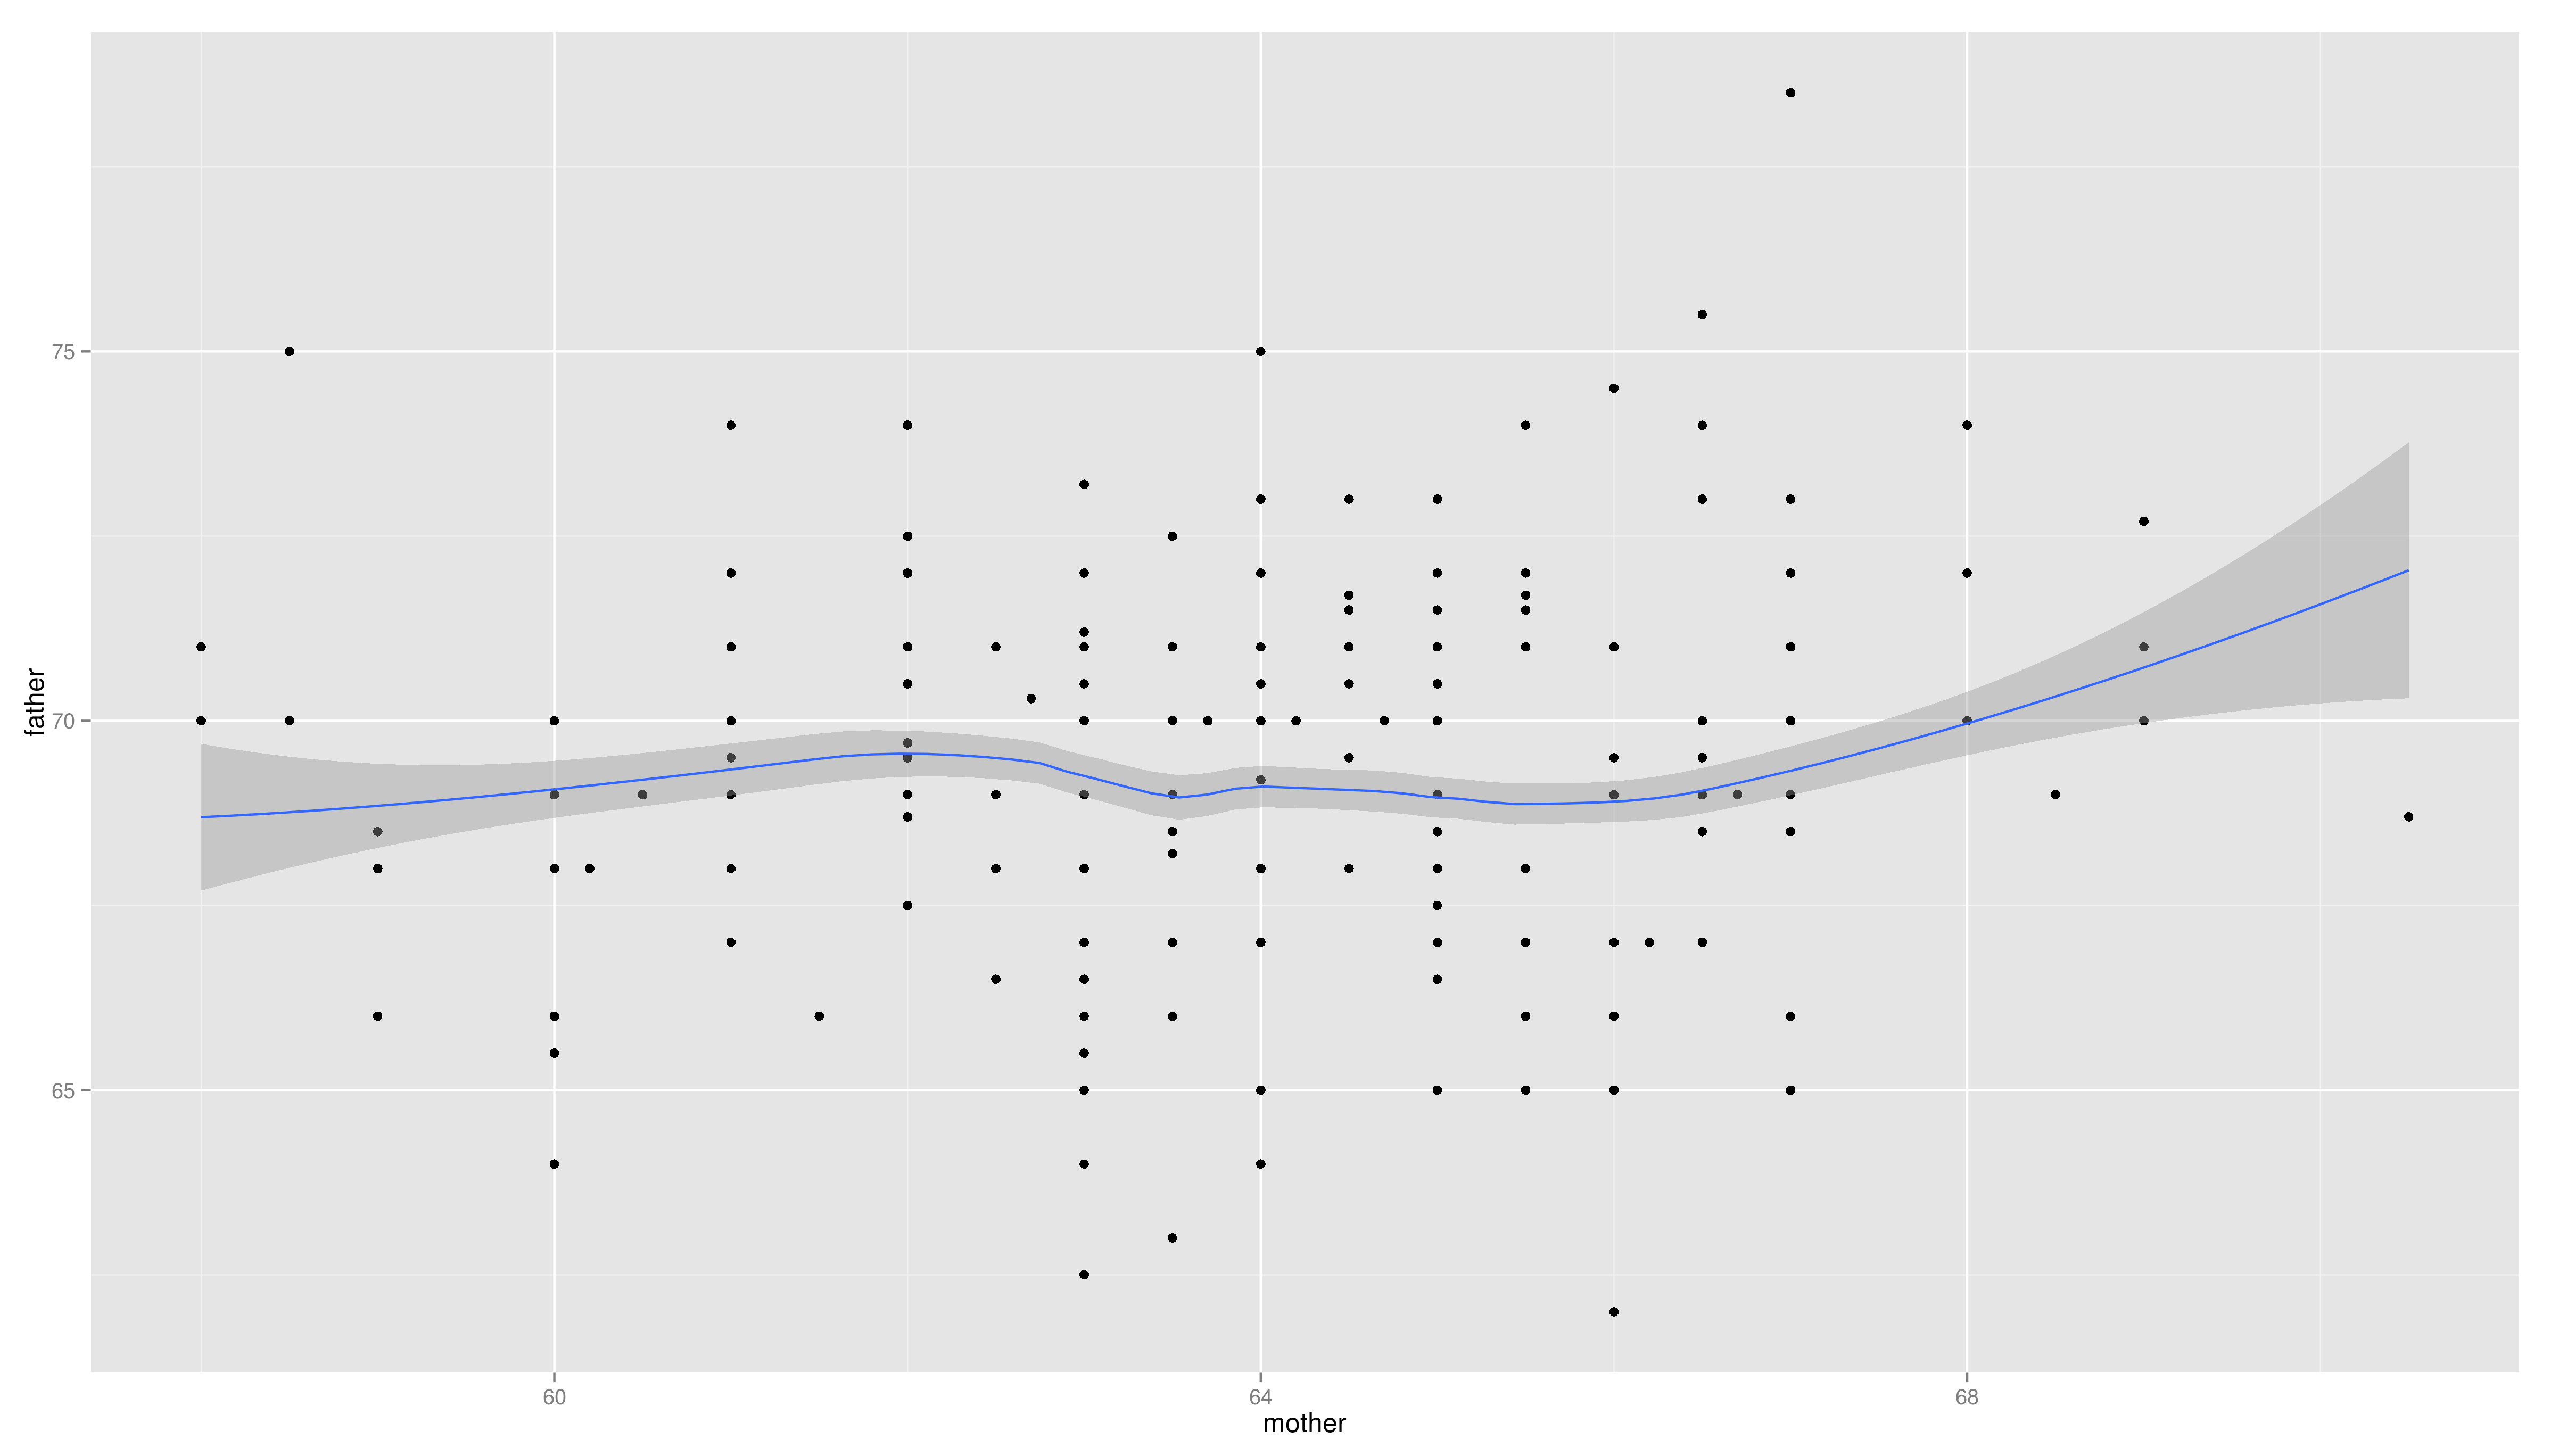
\includegraphics[width=9cm]{scattertrend1.png}
  \end{center}
\end{frame}


\begin{frame}[fragile]\frametitle{Adding trend lines}
  \begin{itemize}
  \item by default \texttt{geom\_smooth()} produces a non-parametric trend line (local polynomial regression fitting for n<1000 otherwise generalized additive model)
  \item we can set a model using the \texttt{method} argument
  \end{itemize}\small
\begin{verbatim}
> ggplot(GaltonFamilies, aes(x=mother,y=father)) +
+     geom_point()
\end{verbatim}
which results in:
\end{frame}


\begin{frame}\frametitle{Adding trend lines}
  \begin{center}
    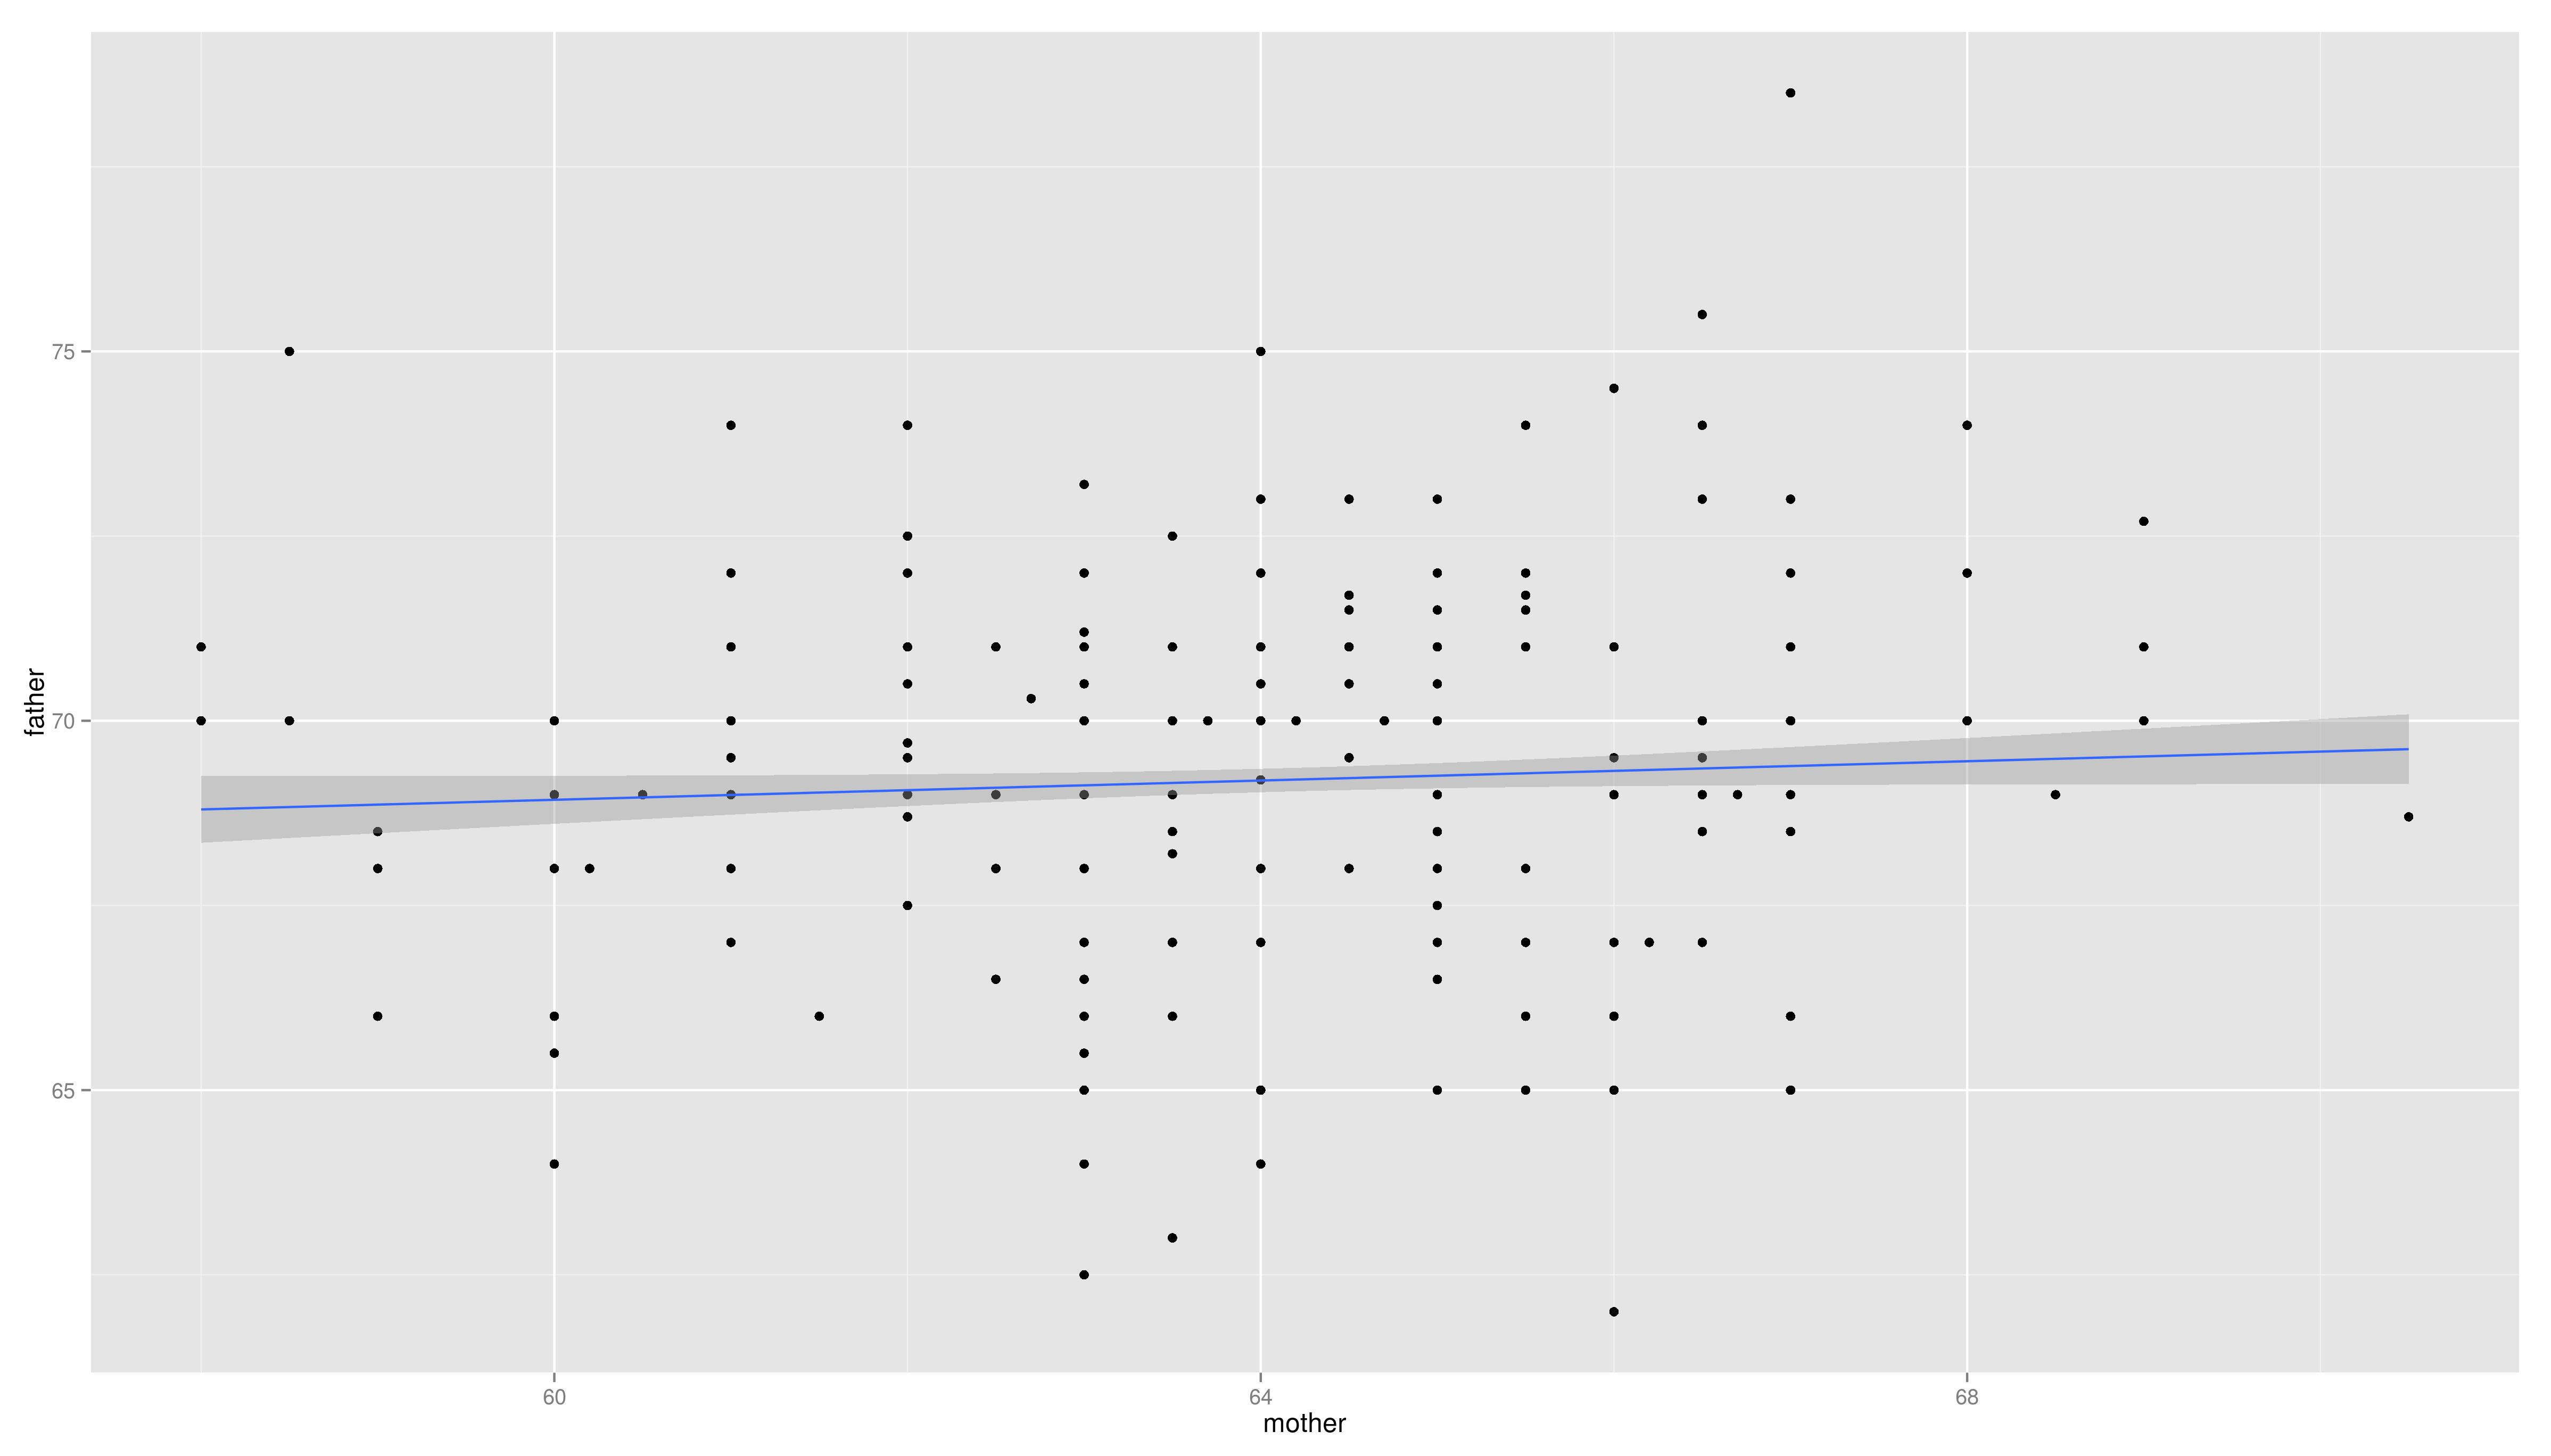
\includegraphics[width=9cm]{scattertrend2.png}
  \end{center}
\end{frame}


\begin{frame}[allowframebreaks]\frametitle{Exercises}
  \begin{enumerate}
  \item use again the GaltonFamilies data set; produce a scatter plot of \texttt{childHeight} vs \texttt{midparentHeight}
  \item add a trend line by using \texttt{geom\_smooth()} without any arguments. Which method is used?
  \item add a second trend line, this time a linear one!
  \item now map the aesthetic \texttt{colour} to \texttt{gender} in the first line of the plot definition. What happens?
  \end{enumerate}
\end{frame}

\end{document}
